\subsection{Explicación formal del problema}

\subsection{Explicación de la solución}

\subsection{Complejidad del algoritmo}

\subsection{Performance del algoritmo}

Como vimos anteriormente, el algoritmo tiene una complejidad de $\Theta(n)$. El algoritmo no tiene peor o mejor caso propiamente dichos (dado que es $\Theta(n)$ para todos los casos), pero veremos que las constantes pueden cambiar para algunas entradas por cuestiones de implementación.

\begin{figure}[H]
 \centering
	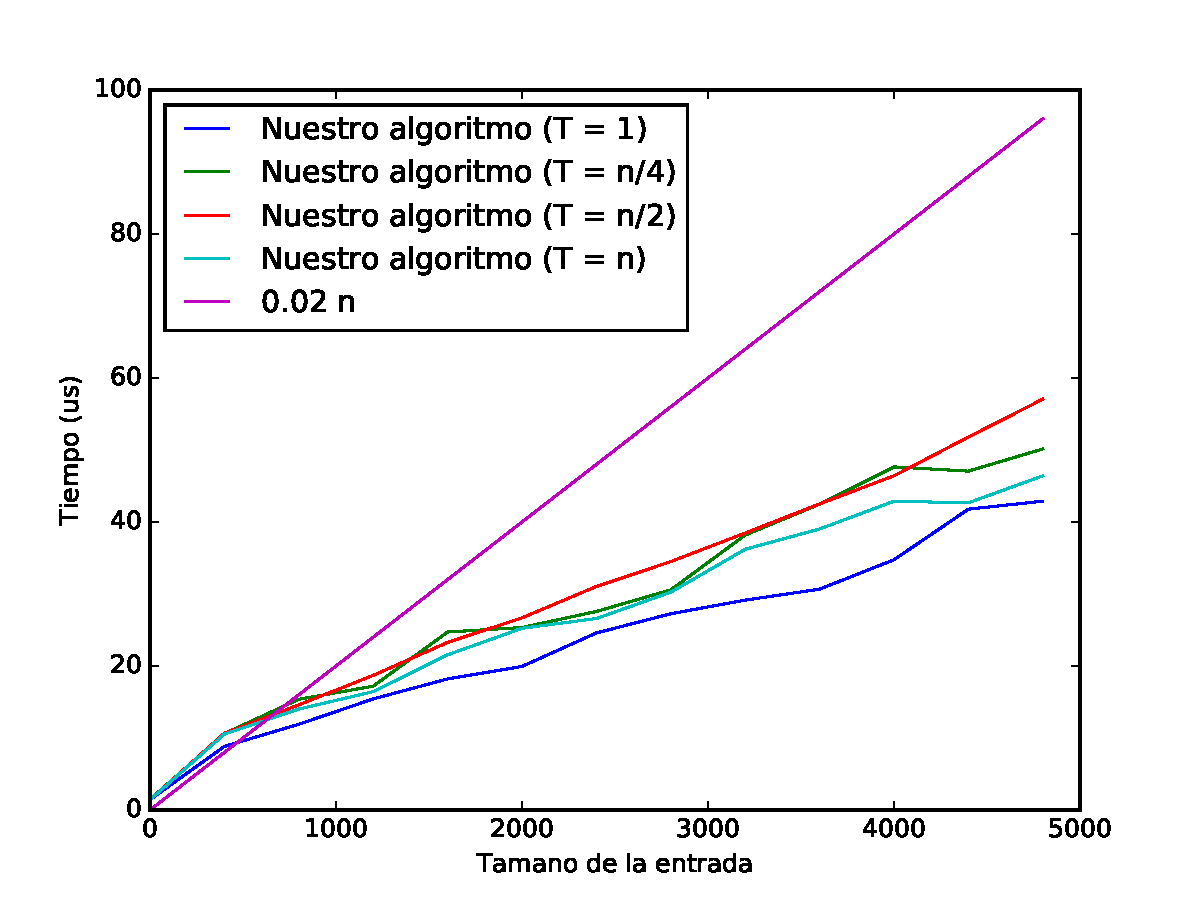
\includegraphics[width=0.8\textwidth]{img/tiempos/genkidama1.pdf}
	\caption{\footnotesize Tiempo que toma el algoritmo en $\mu$s para una entrada de tamaño $n$.}
	\label{fig:genkidama-tiempos1}
\end{figure}

Como se observa, la implementación tiene complejidad lineal, como era esperado. Sin embargo, se observan diferencias según el $T$ que se elija. Recordemos que el $T$ era el radio de impacto del genkidama. Esto se debe a una cuestión de implementacion. Para los casos donde $T = 1$ o $T = n$, nuestra implementación se ahorra entrar a un while, reduciendo la cantidad de instrucciones que ejecuta cada vez.

\begin{figure}[H]
 \centering
	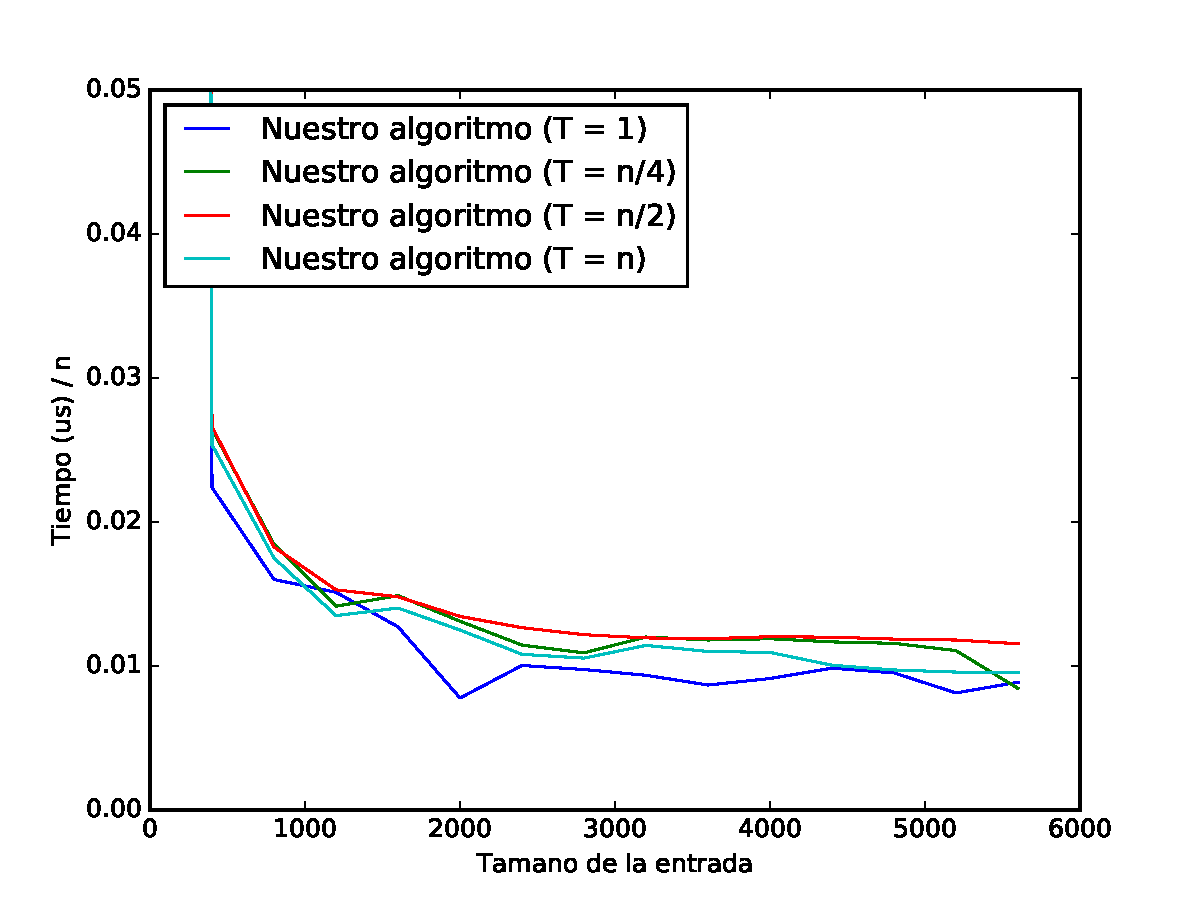
\includegraphics[width=0.8\textwidth]{img/tiempos/genkidama2.pdf}
	\caption{\footnotesize Tiempo que toma el algoritmo en $\mu$s dividido $n$ para una entrada de tamaño $n$.}
	\label{fig:genkidama-tiempos2}
\end{figure}

Este gráfico nos ayuda aún más a confirmar la complejidad lineal de este algoritmo, ayudandonos a ver las constantes para cada caso. Nuevamente, observamos que el caso $T = 1$ tiene una constante un poco menor, debido a lo explicado anteriormente.

Finalmente, veamos que, para instancias de igual tamaño, el tiempo que se tarda en resolverlas no varía demasiado (confirmando el hecho de que para $T$ fijo, la elección de los puntos no cambia el tiempo de ejecución de manera significativa).

\begin{figure}[H]
 \centering
	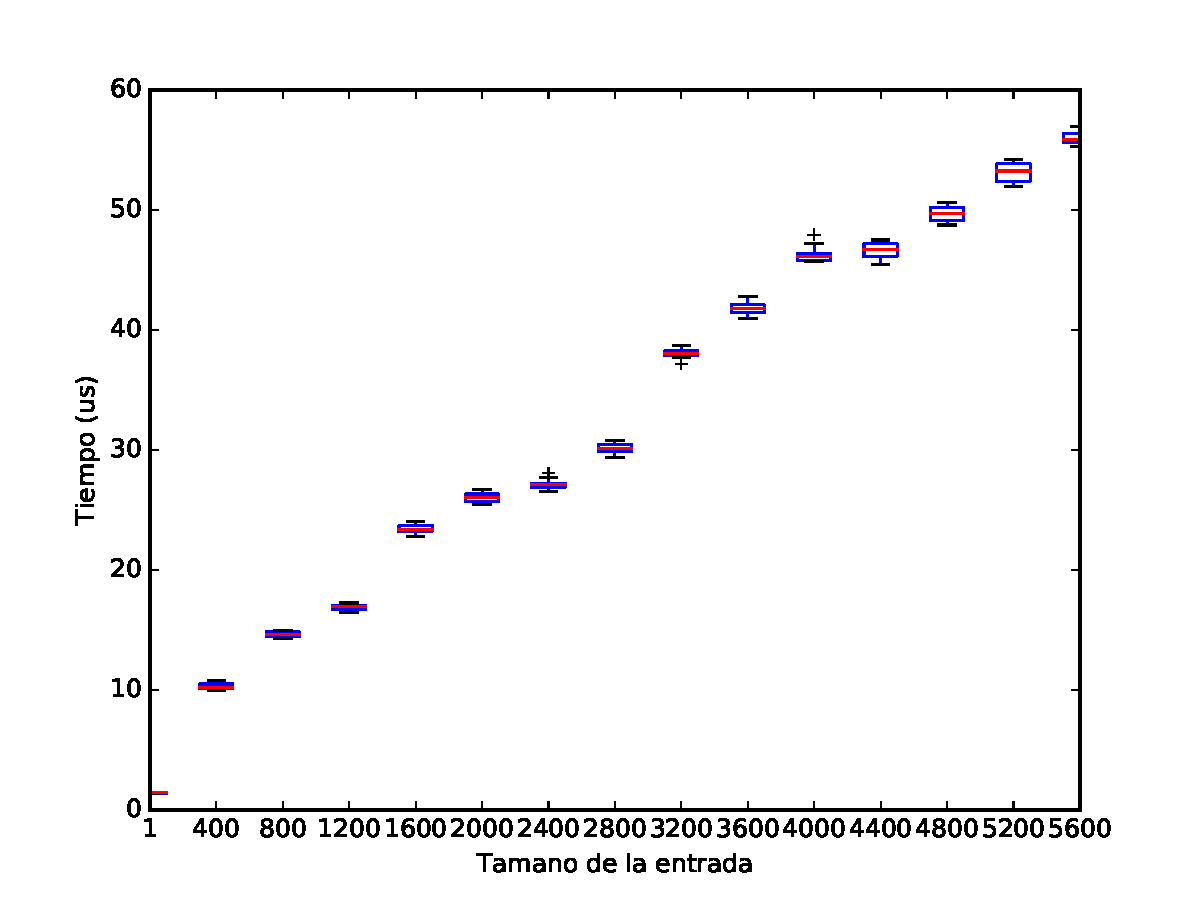
\includegraphics[width=0.8\textwidth]{img/tiempos/genkidama3.pdf}
	\caption{\footnotesize Tiempo que toma el algoritmo en $\mu$s para una entrada de tamaño $n$. $T = n/4$. Se indican los valores del primer al tercer cuatril con un rectángulo azul y la mediana con una linea roja. El máximo y minimo se indican con lineas negras arriba y abajo del rectángulo.}
	\label{fig:genkidama-tiempos3}
\end{figure}

\subsubsection{M\'etodo de experimentación}

Para los primeros dos gráficos (es decir, para la figura \label{fig:genkidama-tiempos1} y la figura \label{fig:genkidama-tiempos2}), generamos 50 instancias al azar de para cada $n$.
Las instancias fueron generadas de la siguiente manera: para cada $n$, elegimos $n$ puntos al azar de la grilla $\{1,..., n^2\} \times \{1, ... , n^2\}$.
Estos puntos eran elegidos al azar usando el mismo \emph{seed} cada vez (para la instancia 1 usabamos 1 como seed, para la instancia 2, usabamos 2, etc.), de tal manera que los experimentos fueran reproducibles de una manera válida.

Cada instancia fue ejecutada 20 veces, y el resultado final era el mínimo de todas las corridas.
Luego, tomabamos la mediana de todas las instancias.
Es decir, el restultado final es la mediana de los mínimos. Como puede observarse en la figura \ref{fig:genkidama-tiempos3}, la mediana es muy representativa de lo que sucede.
